\documentclass[border = 5pt, tikz]{standalone}
\usepackage{styles}
\usepackage{tikz}
\usetikzlibrary{calc}


\newcommand\s{2cm}
\begin{document}
  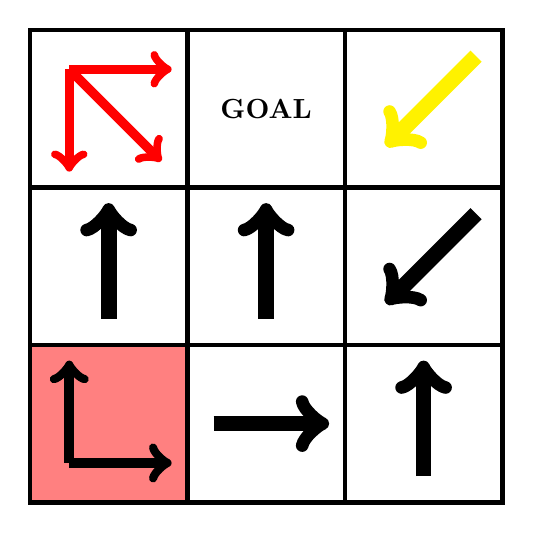
\begin{tikzpicture}[
      state/.style = {
        draw=black,
        ultra thick,
        minimum size = \s,
      },
      arr/.style = {
        draw=black,
        ultra thick,
        ->,
        line width=1.2mm,
      },
    ]
      \node[state] (11) at (0, 0) {};
      \node[state] (12) at (\s, 0) {\textbf{GOAL}};
      \node[state] (13) at (2*\s, 0) {};
      \node[state] (21) at (0, -\s) {};
      \node[state] (22) at (\s, -\s) {};
      \node[state] (23) at (2*\s, -\s) {};
      \node[state, fill=red!50!white] (31) at (0, -2*\s) {};
      \node[state] (32) at (\s, -2*\s) {};
      \node[state] (33) at (2*\s, -2*\s) {};
      \draw[arr, red] ($(11.center) + (-\s/4, \s/4)$) -- +(\s/2.5+\s/4, 0);
      \draw[arr, red] ($(11.center) + (-\s/4, \s/4)$) -- +(0, -\s/2.5-\s/4);
      \draw[arr, red] ($(11.center) + (-\s/4, \s/4)$) -- +(\s/3 + \s/4, -\s/3 - \s/4);
      \draw[arr, line width=2mm, yellow] ($(13.center) + (\s/3, \s/3)$) -- +(-2*\s/3.5, -2*\s/3.5);
      \draw[arr, line width=2mm] ($(21.center) + (0, -\s/3)$) -- +(0, \s/3 + \s/2.5);
      \draw[arr, line width=2mm] ($(22.center) + (0, -\s/3)$) -- +(0, \s/3 + \s/2.5);
      \draw[arr, line width=2mm] ($(23.center) + (\s/3, \s/3)$) -- +(-2*\s/3.5, -2*\s/3.5);
      \draw[arr, line width=1.3mm] ($(31.center) + (-\s/4, -\s/4)$) -- +(0, \s/4 + \s/2.5);
      \draw[arr, line width=1.3mm] ($(31.center) + (-\s/4, -\s/4)$) -- +(\s/2.5+\s/4, 0);
      \draw[arr, line width=2mm] ($(32.center) + (-\s/3, 0)$) -- +(\s/2.5 + \s/3, 0);
      \draw[arr, line width=2mm] ($(33.center) + (0, -\s/3)$) -- +(0, \s/3 + \s/2.5);

    \end{tikzpicture}
\end{document}